\par{This kernel is as far as we know, the most straightforward implementation of matrix matrix multiplication kernel.
    Optimisations were not implemented on this kernels as it can be seen in listing \ref{naive_kernel}. Every instance
    of the kernel calculates one element of the output matrix.}

\lstinputlisting[float,caption={Naive kernel.}, label={naive_kernel}, 
                style=customc]{/Users/clalanne/GitHubProjects/OpenCLNotes/src/code/naive.c}

\par{The results executing this kernel in different architectures with different number of \emph{work groups } can be seen 
in figure \ref{Naive}. From these figures we can notice immediatelly that using \emph{work groups} larger than or equal than 16
\emph{work items} in the dimension 0 speedups the execution of the kernel roughly 8 times in the case of Intel Xeon Phi.
Xeon shows the same trend but with an smaller speedup 3.5 approximately.}

\lstinputlisting[float,caption={Naive kernel LLVM code Xeon.}, label={llvm_code_naive_cpu}, 
                style=customc]{/Users/clalanne/GitHubProjects/OpenCLNotes/src/code/llvm_naive_cpu.ll}

\lstinputlisting[float,caption={Naive kernel LLVM code Intel Xeon Phi.}, label={llvm_code_naive_phi}, 
                style=customc]{/Users/clalanne/GitHubProjects/OpenCLNotes/src/code/llvm_naive_phi.ll}

\par{This could be explained in both cases by what the compiler and the run-time trying to do in terms of vectorization. In both 
cases these numbers fit the vectorization that the compiler is trying to achieved, listings 
\ref{llvm_code_naive_cpu} and \ref{llvm_code_naive_phi}, shows the type of LLVM instructions that the intel compiler is using to 
vectorize operations, its possible to see that the Xeon cpu is using a factor of 4 and the Intel Xeon Phi is using a factor of 16.}

\par{Another important issue to notice is that as you would assume theoretically the gathering of elements to fill the vector 
units on the Intel Xeon Phi seems to take almost of the time of the kernel as we can see in figure \ref{vtune_naive}.}

\begin{figure}[!h]
    \centering
    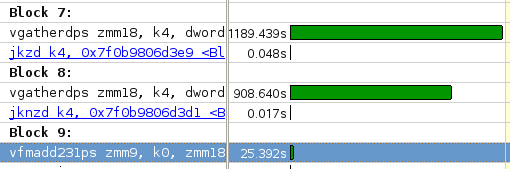
\includegraphics[width=0.49\textwidth]{figures/vtune_naive.png}
    \caption{Vtune profiler in the native kernel.}
    \label{vtune_naive}
\end{figure}

\par{Also figure \ref{Naive} shows that not in all of the \emph{work group} sizes it is possible to execute the kernel in the GPU. 
This is because the GPU run out of resources in those cases\cite{opencl_error} as its possible to see in figure 
\ref{GpuDeviceInfo}.}

\par{Reading the kernel\ref{naive_kernel}, its possible to see that there is no effort to use caches efficiently, locality of
memory access pattern its far from ideal in the top of this the gathering of data from memory force to have a high CPI(clock per
instructions). This is true even in the Xeon and Intel Xeon Phi architecture even though both count with a automatic caching system.}

\par{Figure \ref{NaiveComp} shows that GPUs achived the best performance in comparison with the other architectures. This is 
    reasonable and it was expected for the kernels studied in this report. The reason is because you can think on the model of vector
    execution of the Xeon Phi and the Xeon as smaller \emph{warps} in this sense the GPU can execute wider and more \emph{warps} in
    parallel than the other 2 architectures.}
    
\par{In this case in particular the gpu is faster than the other architectures when the \emph{work group} size is 1x1024 
    , it is interesting to observe that in this case the with a \emph{work group} size of 1x1024 is faster than 1024x1,this is 
    mainly because with 1x1024 the memory access pattern to the matrix B its coalesced which does not happen when the \emph{
        work group} dimension is 1024x1.}

\begin{figure}[!h]
    \centering
    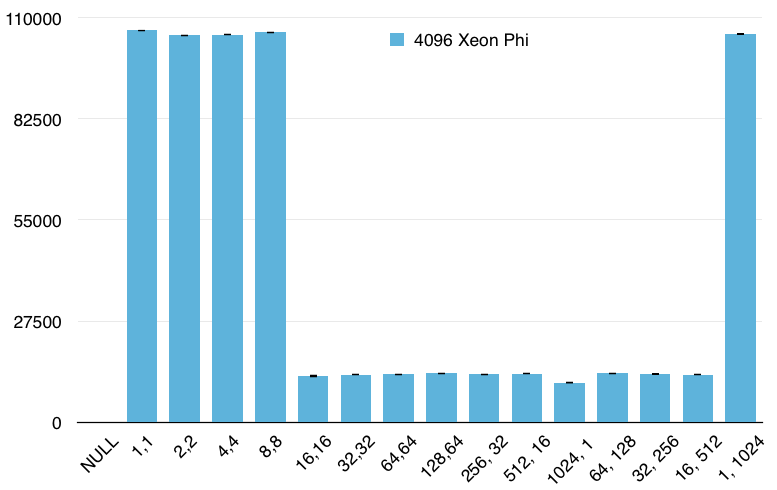
\includegraphics[width=0.49\textwidth]{figures/naive_phi.png}
    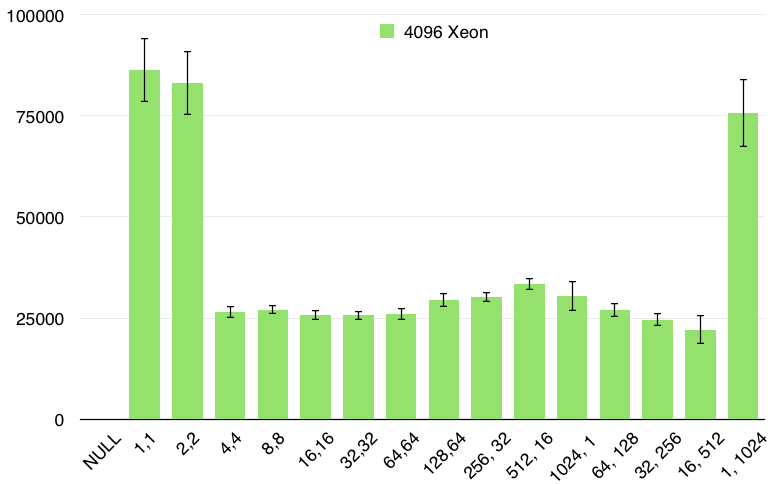
\includegraphics[width=0.49\textwidth]{figures/naive_cpu.png}
    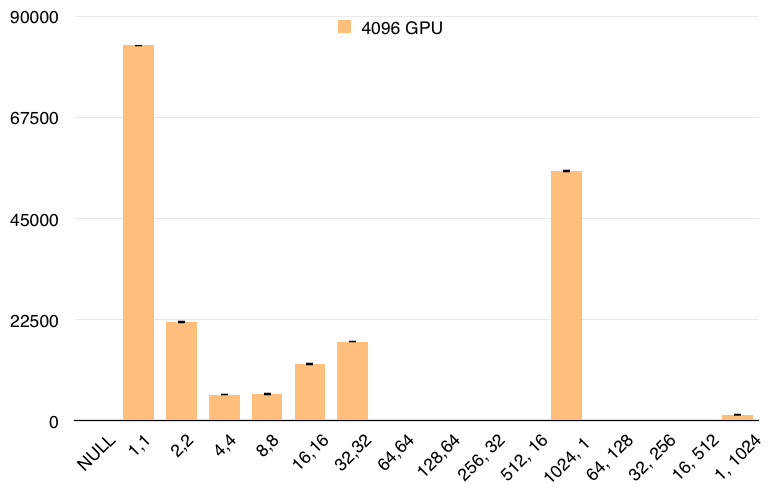
\includegraphics[width=0.49\textwidth]{figures/naive_gpu.png}
    \caption{Naive matrix multiplication in different architectures.}
    \label{Naive}
\end{figure}

\begin{figure}[!h]
    \centering
    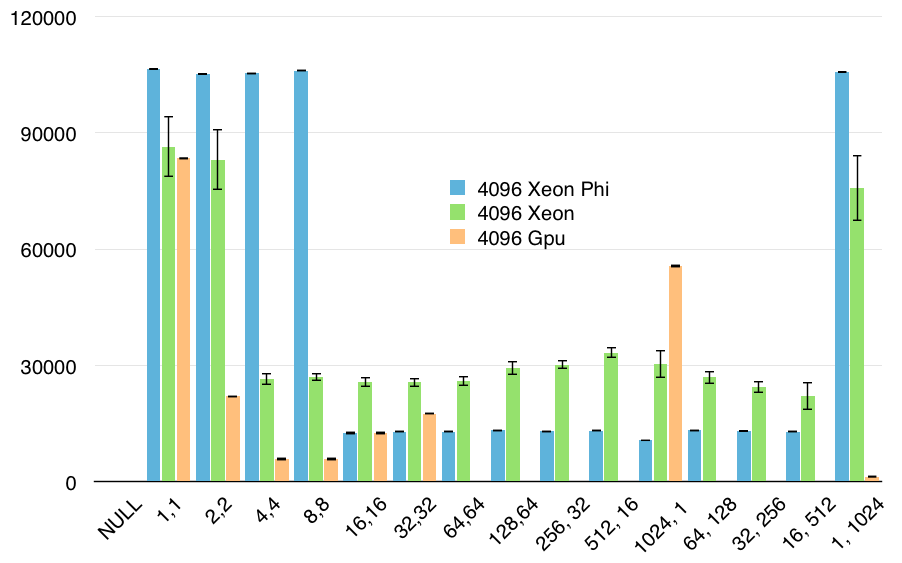
\includegraphics[width=0.6\textwidth]{figures/naive_comp.png}
    \caption{Naive matrix multiplication in different architectures comparison.}
    \label{NaiveComp}
\end{figure}

